\documentclass[12pt]{book}
\usepackage{graphicx}
\usepackage{amsmath,amssymb,fullpage,cancel,hyperref}
\usepackage{tikz,tcolorbox}
\usepackage[miktex]{gnuplottex}
\usepackage{titlesec}
\usepackage[Bjornstrup]{fncychap}
\usepackage{lscape}
\usepackage{import}
\usepackage{breqn}
\tcbuselibrary{theorems}
\newcommand{\ds}{\displaystyle}
\allowdisplaybreaks
\setcounter{tocdepth}{4}
\setcounter{secnumdepth}{4}
\usepackage[titles]{tocloft}
\makeatletter
\newcommand*{\tocwithouttitle}{\@starttoc{toc}}
\makeatother
\usepackage{pgfplots, pgfplotstable}
\pgfplotsset{compat=1.8}

\renewcommand{\labelitemii}{$\diamond$}

\newcommand{\sep}{\vskip .7in}
\newcommand{\ansbox}[1]{%
\hbox to 1.5 truein{\hfil \framebox{\parbox[b]{#1in}{\quad \\ \quad}}}}
%%%%%%%%%%%%%%%%%%%%%%%%%%%%%%%%%%%%%%%%%%%%%%%%%%%%%%%%%%%%%%%%%%%%%%%%%
\baselineskip =20pt
\parskip =10pt
\newcommand{\ts}{\textsuperscript}
\newtheorem{theorem}{Theorem}
\newtheorem{alg}{Algorithm}
\newtheorem{case}{Case}
\newtheorem{scase}{Case}[case]
\newtheorem{sscase}{Case}[scase]
\newtheorem{ssscase}{Case}[sscase]
\newtheorem{sssscase}{Case}[ssscase]
\newtheorem{claim}{Claim}
\newtheorem{prop}{Proposition}
\newtheorem{cor}{Corollary}
\newtheorem{defn}{Definition}
\newtheorem{lemma}{Lemma}
\newtheorem{note}{Note}
\newtheorem{fact}{Fact}
\newtheorem{game}{Game}
\newtheorem{strat}{Strategy}
\newtheorem{ex}{Example}
\newtheorem{prob}{Problem}
\newtheorem{subprob}{Sub-Problem}
\newtheorem{subsubprob}{Sub-Sub-Problem}
\newtheorem{rul}{Rule}
\newtheorem{remark}{Remark}
\newtheorem{objec}{Objective}
\newtheorem{hwk}{Homework}
\newtheorem{step}{Step}
\newtheorem{rvw}{Review}
\numberwithin{subprob}{prob}
\numberwithin{subsubprob}{subprob}
\renewcommand\thesubprob{\Alph{subprob}}

%**********Highlighted Theorems and Defs**********
\newtcbtheorem{imp:thm}{Theorem}%
{colback=blue!5,colframe=blue!35!black,fonttitle=\bfseries}{th}
\newtcbtheorem{imp:defn}{Definition}%
{colback=blue!5,colframe=blue!35!black,fonttitle=\bfseries}{th}
\newtcbtheorem{imp:rule}{Rule}%
{colback=blue!5,colframe=blue!35!black,fonttitle=\bfseries}{th}
\newtcbtheorem{imp:form}{Formula}%
{colback=blue!5,colframe=blue!35!black,fonttitle=\bfseries}{th}
\newtcbtheorem{imp:ex}{Example}%
{colback=blue!5,colframe=blue!35!black,fonttitle=\bfseries}{th}
%*************************************************

\newenvironment{sol}%
{%
\noindent{\it Solution.}
}%
{%
 \quad\hfill$\blacktriangledown$\vspace*{2ex}
}

%***Graphing Code
%\begin{tikzpicture}[domain=-2:3,xscale=.6,yscale=.6]
%\draw[thin,color=gray!40] (-2.1,-2.1) grid (3.1,8.1);
%\draw[->,thick] (-2.2,0) -- (3.2,0) node[right] {x};
%\draw[->,thick] (0,-2.2) -- (0,8.2) node[above] {y};
%\draw[thick,color=blue,domain=-2:3,samples=200] plot[id=ex1a] function{(x-1)**2-1} node[right] {$f$};
%\end{tikzpicture}

\title{MAT 350 - Applied Linear Algebra}
\author{Mr. Ryan Evaul\\
Southern New Hampshire University}

\begin{document}
%\frontmatter
\maketitle
%\tableofcontents

\chapter*{\contentsname}
\markboth{\MakeUppercase{\contentsname}}{\MakeUppercase{\contentsname}}
\tocwithouttitle
%\begin{landscape}
% !TEX root = /Users/us2009801/Documents/GitHub/LinearAlgebra/main.tex
\chapter{Class 1 - Thursday, September 19\ts{th}, 2017}
\section{\S 1 Differential Equations}


$$
\begin{bmatrix}
    x_{11}       & x_{12} & x_{13} \\
    x_{21}       & x_{22} & x_{23} \\
\end{bmatrix}
$$
% !TEX root = /Users/us2009801/Documents/GitHub/LinearAlgebra/main.tex
\chapter{Class UNK - Monday, October 23\ts{rd}, 2017}
\section{\S 2.8 Subspaces}

\begin{imp:defn}{Subspace}{} A subspace of rton is any set H in  that has three properties:
\begin{itemize}
  \item  is in H
  \item For each u, v, in H u+v is also in H (Closure under addition)
  \item For each u in H and scalar C, cu is in H (Closure under scalar multiplication)
\end{itemize}
\end{imp:defn}
\begin{ex}
%image
fdsaf
Is H a subspace of rto2?
\begin{itemize}
\item is in h \checkmark
\item u+v is not in H for all u,v in H
\item Not closed under scalar multiplication either (-u not in H).
\end{itemize}
H is not a subspace
\end{ex}
\begin{ex}
%image
\begin{itemize}
    \item is in H \checkmark
    \item closed under addition \checkmark
    \item closed under scalar multiplication \checkmark
\end{itemize}
H is a subspace of rto2
\end{ex}
\begin{ex}
Which of the following are subspaces of $\mathbb{R}^{2}$?

\begin{itemize}
    \item %image\\
    not a subspace o is not in h
    \item %imgae\\
    $\mathbb{R}^2$ is a subspace of $\mathbb{R}^2$
    \item %image\\
    $\mathbb{R}^2$ is a subspace of $\mathbb{R}^2$
    \item %image\\
    \begin{itemize}
        \item o is in H \checkmark
        \item Closed under scalar multiplicaiton \checkmark
        \item Not closed unfer addition x u+(-v) in in H.
    \end{itemize}
    not a subspace of $\mathbb{R}^2$
    \item %image% 
    stuff
\end{itemize}
\end{ex}
So what are do subspaces of $\mathbb{R}^2$ look like?
\begin{itemize}
    \item They are copies of $\mathbb{R}^0$, $\mathbb{R}^1$, $\mathbb{R}^2$... $\mathbb{R}^n$ that contain the zero vector.
\end{itemize}
\begin{ex}
In $\mathbb{R}^3$, possible subspaces are:
\begin{itemize}
    \item Zero Subspaces
    \item Lines
    \item Planes
\end{itemize}
\end{ex}
\begin{ex}
If H=span{$v_1$,$v_2$} ({$av_1$,$bv_2$} for any a,b), then H is a subspace of $\mathbb{R}^n$
\begin{itemize}
\item o is in H \checkmark
\begin{itemize}
    \item since o*$v_1$ +o*$v_2$=o
\end{itemize}
\item closed under addition \checkmark
\begin{itemize}
    \item $u=a_1v_1+b_1v_2$
    \item $w=a_2v_1+b_2v_2$
    \item $u+w=a_1v_1+b_1v_2+a_2v_1+b_2v_2$
    \item $u+w=(a_1+a_2)v_1+(b_1+b_2)v_2$
    \item which is span{$v_1$,$v_2$}
\end{itemize}
\item closed under scalar multiplication
\begin{itemize}
    \item $u=av_1+bv_2$
    \item $c*u=c(av_1+bv_2)=(c*a)v_1+(c*b)v_2$
\end{itemize}
which is span{$v_1$,$v_2$}
\end{itemize}
\end{ex}
\begin{imp:defn}{Column Space}{} The column space of a matrix A, denoted col(A), is the set of all linear combinations of the columns of A. (col(a) is a subspace)
\end{imp:defn}
\begin{ex}
Let $A=
\begin{bmatrix}
   1 & -3 & -4\\
   -4 & 6 & -2\\
   -3 & 7 & 6\\
\end{bmatrix}
$ and $b= 
\begin{bmatrix}
   3 \\
   3 \\
   -4\\
\end{bmatrix}$\\
is b in Col(A)?\\
if b is a linear combination of the columns of A,
the Ax=b has a solution. We are asking whether [A|b] is consistant of not.\\
$
\begin{bmatrix}
   1 & -3 & -4 & | & 3\\
   -4 & 6 & -2 & | & 3\\
   -3 & 7 & 6 & | & -4\\
\end{bmatrix}
$ goes to $
\begin{bmatrix}
   1 & -3 & -4 & | & 3\\
   0 & -6 & -18 & | & 15\\
   0 & 0 & 0 & | & 0\\
\end{bmatrix}
$\\
No pivot in augmented column, so b is in col(A).\\
Note: b in col(A) for every b in $\mathbb{R}^m$\\
\begin{itemize}
    \item Ax=b has a solution for every b in $\mathbb{R}^m$
    \item The columns of A span $\mathbb{R}^m$
    \item A has a pivot in every row in REF
\end{itemize}
\end{ex}
\begin{imp:defn}{Null Space}{} The null space of matrics A, denoted null(A), is the set of all solutions to Ax=$\vec o$
\end{imp:defn}
\begin{note} Any solution set of Ax=$\vec o$ can be written in parametric form.\\
$x=x_2\begin{bmatrix}
0\\
2\\
1\\
\end{bmatrix} + x_3 \begin{bmatrix}
0\\
0\\
1\\
\end{bmatrix} =$span$ \{ \begin{bmatrix}
0\\
2\\
1\\
\end{bmatrix} \begin{bmatrix}
0\\
0\\
1\\
\end{bmatrix} \}$\\
so null(A) is a subspace.
\end{note}
\begin{imp:defn}{Basis for a Subspace}{} A basis for a subspace H is a linearly independent set that spans H.
\end{imp:defn}
\begin{ex}
Find a basis for null(A), if
$A=\begin{bmatrix}
-3 & 6 & -1 & 1 &-7\\
1 & -2 & 2 & 3 & -1\\
2 & -4 & 5 & 8 &-4 \\
\end{bmatrix}$\\
$A=\begin{bmatrix}
1 & -2 & 0 & -1 & -3 & | & 0\\
0 & 0 & 1 & 2 & -2 & | & 0\\
0 & 0 & 0 & 0 & 0  & | & 0\\
\end{bmatrix}$
\begin{align*}
    x_1-2x_2-x_4+3x_5&=0\\
    x_2&=x_2\\
    x_3+2x_4-2x_5&=0\\
    x_4&=x_4\\
    x_5&=x_5
\end{align*}

\end{ex}
\chapter{Test 01 Corrections}

\begin{prob} 10pts
\begin{subprob}
Correct
\end{subprob}
\begin{subprob}
Correct
\end{subprob}
\end{prob}
\begin{prob}
$A=
\begin{bmatrix}
   1 & 2 & 1\\
   -3 & -1 & 2\\
   0 & 5 & 3\\
\end{bmatrix}$ and $B=\begin{bmatrix}
   0 \\
   5 \\
   -1 \\
\end{bmatrix}$\\
\begin{align*}
&\begin{bmatrix}
   1 & 2 & 1 & | & 0\\
   -3 & -1 & 2 & | & 5\\
   0 & 5 & 3 & | & -1\\
\end{bmatrix}\\
r_2\rightarrow r_2+3r_1&\begin{bmatrix}
   1 & 2 & 1 & | & 0\\
   0 & 5 & 5 & | & 5\\
   0 & 5 & 3 & | & -1\\
\end{bmatrix}\\
r_2\rightarrow r_2/5&\begin{bmatrix}
   1 & 2 & 1 & | & 0\\
   0 & 1 & 1 & | & 1\\
   0 & 5 & 3 & | & -1\\
\end{bmatrix}\\
r_3\rightarrow r_3-5r_2&\begin{bmatrix}
   1 & 2 & 1 & | & 0\\
   0 & 1 & 1 & | & 1\\
   0 & 0 & -2 & | & -6\\
\end{bmatrix}\\
r_3\rightarrow r_3/-2&\begin{bmatrix}
   1 & 2 & 1 & | & 0\\
   0 & 1 & 1 & | & 1\\
   0 & 0 & 1 & | & 3\\
\end{bmatrix}\\
r_1\rightarrow r_1-2r_2&\begin{bmatrix}
   1 & 0 & -1 & | & -2\\
   0 & 1 & 1 & | & 1\\
   0 & 0 & 1 & | & 3\\
\end{bmatrix}\\
r_1\rightarrow r_1+r_3&\begin{bmatrix}
   1 & 0 & 0 & | & 1\\
   0 & 1 & 1 & | & 1\\
   0 & 0 & 1 & | & 3\\
\end{bmatrix}\\
r_2\rightarrow r_2-r_3&\begin{bmatrix}
   1 & 0 & 0 & | & 1\\
   0 & 1 & 0 & | & -2\\
   0 & 0 & 1 & | & 3\\
\end{bmatrix}\\
\end{align*}
Yes, B is in the subset spanned by the columns of A.
$$0\begin{bmatrix}
   1 \\
   -3 \\
   0 \\
\end{bmatrix}+5\begin{bmatrix}
   2 \\
   -1 \\
   5 \\
\end{bmatrix}-1\begin{bmatrix}
   1 \\
   2 \\
   3 \\
\end{bmatrix}=\begin{bmatrix}
   1 \\
   -2 \\
   3 \\
\end{bmatrix}$$
\end{prob}
\begin{prob}
Yes, the figure does have a solution; if you express the vectors as a linear combination $x_1v_1+x_2v_2+x_3v_3=b$ you can change the values of the scalars ($x_1$, $x_2$, $x_3$) to any value which, when multiplied by the vectors will give us any b; which causes the answer to b to be non-unique.

\begin{center}
    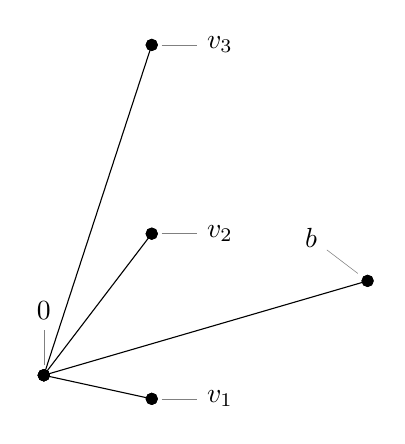
\begin{tikzpicture}
\begin{axis}[
    hide axis,
    xmin=-1, xmax=4,
    ymin=-1.5, ymax=8,
]
 
 \addplot[mark=*] coordinates {(0,0)} node[pin=90:{$0$}]{};
  \addplot[mark=*] coordinates {(1,7)} node[pin=0:{$v_3$}]{};
   \addplot[mark=*] coordinates {(3,2)} node[pin=150:{$b$}]{};
      \addplot[mark=*] coordinates {(1,-.5)} node[pin=0:{$v_1$}]{};
         \addplot[mark=*] coordinates {(1,3)} node[pin=0:{$v_2$}]{};
\addplot[mark=oplus] coordinates {(0,0)(1,7) };
    \addplot[mark=oplus] coordinates {(0,0)(1,3)};
    \addplot[mark=oplus] coordinates {(0,0)(3,2)};
 \addplot[mark=oplus] coordinates {(0,0)(1,-.5)};
\end{axis}
\end{tikzpicture}
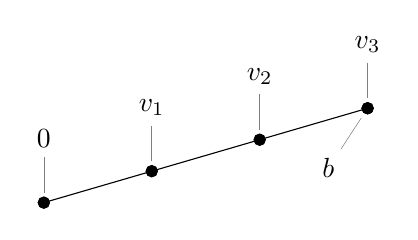
\begin{tikzpicture}
\begin{axis}[
    hide axis,
    xmin=-1, xmax=4,
    ymin=-1.5, ymax=8,
]
 
 \addplot[mark=*] coordinates {(0,0)} node[pin=90:{$0$}]{};
  \addplot[mark=*] coordinates {(3,2)} node[pin=90:{$v_3$}]{};
   \addplot[mark=*] coordinates {(3,2)} node[pin=240:{$b$}]{};
      \addplot[mark=*] coordinates {(1,2/3)} node[pin=90:{$v_1$}]{};
         \addplot[mark=*] coordinates {(2,4/3)} node[pin=90:{$v_2$}]{};
\addplot[mark=*] coordinates {(0,0)(1,2/3)(2,4/3)(3,2) };
\end{axis}
\end{tikzpicture}
\end{center}
\end{prob}
\begin{prob} 10pts
\begin{subprob}
\begin{align*}
&\begin{bmatrix}
   1 & 3 & 1\\
   0 & 3 & 6\\
   0 & 0 & 0\\
\end{bmatrix}\\
r_1\rightarrow r_1-r_2&\begin{bmatrix}
   1 & 0 & -5\\
   0 & 3 & 6\\
   0 & 0 & 0\\
\end{bmatrix}\\
r_2\rightarrow r_2/3&\begin{bmatrix}
   1 & 0 & -5\\
   0 & 1 & 2\\
   0 & 0 & 0\\
\end{bmatrix}\\
1x_1-5x_3&=0\\
1x_2+2x_3&=0\\
x_1&=5x_3\\
x_2&=-2x_3\\
x_3&=x_3\\
\begin{bmatrix}
   x_1\\
   x_2\\
   x_3\\
\end{bmatrix}&=\begin{bmatrix}
   5x_3\\
   -2x_3\\
   0\\
\end{bmatrix}\\
\begin{bmatrix}
   5x_3\\
   -2x_3\\
   0\\
\end{bmatrix}&=x_3\begin{bmatrix}
   5\\
   -2\\
   0\\
\end{bmatrix}
\end{align*}
\end{subprob}
\begin{subprob}
$$0\begin{bmatrix}
   5\\
   -2\\
   0\\
\end{bmatrix} = \begin{bmatrix}
   0\\
   0\\
   0\\
\end{bmatrix}$$
\end{subprob}
\begin{subprob}
Yes, $x_3$ is a free variable, any value will have a solution.
\end{subprob}
\end{prob}
\begin{prob} 30pts
\begin{subprob}
Correct
\end{subprob}
\begin{subprob}
Yes, because there is no way to reduce the matrices to be in the other matrix.
\end{subprob}
\begin{subprob}
No, it is linearly dependent because $v_1$, $v_2$ are dependant.
\end{subprob}
\begin{subprob}
No, because the vectors are not necessarily related.
\end{subprob}
\begin{subprob}
Yes, because the columns are related and a part of the same system.
\end{subprob}
\begin{subprob}
Yes, there are pivots in each column and there is no free variable therefore the sets are independant of each other.
\end{subprob}
\end{prob}
\begin{prob}
$\begin{bmatrix}
   2\\
   0\\
\end{bmatrix}-3\begin{bmatrix}
   3\\
   2\\
\end{bmatrix}=\begin{bmatrix}
   2\\
   0\\
\end{bmatrix}-\begin{bmatrix}
   9\\
   6\\
\end{bmatrix}=\begin{bmatrix}
   -7\\
   -6\\
\end{bmatrix}$
\end{prob}
\begin{prob} 10pts
\begin{center}
    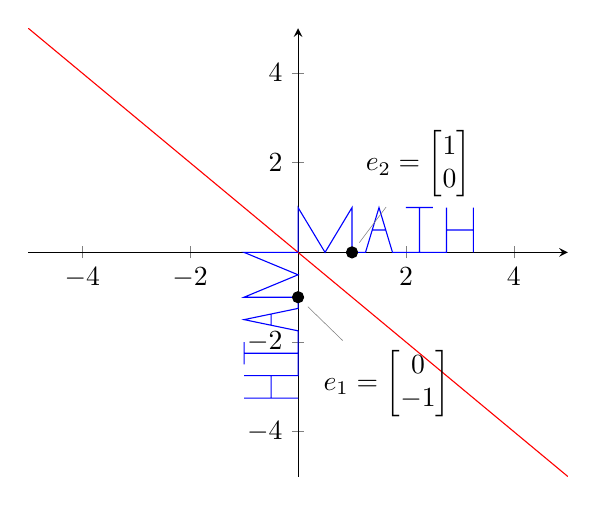
\begin{tikzpicture}
\begin{axis}[
axis lines = center,
    xmin=-5, xmax=5,
    ymin=-5, ymax=5,
]
 
\addplot [
    domain=-10:10, 
    samples=100, 
    color=red,
]
{-x};
\addplot[
    color=blue,
    ]
    coordinates {
    (0,0)(0,1)(0.5,0)(1,1)(1,0)(1.25,0)(1.5,1)(1.75,0)(1.625,0.5)(1.375,0.5)(1.625,0.5)(1.75,0)(2.25,0)(2.25,1)(2,1)(2.5,1)(2.25,1)(2.25,0)(2.75,0)(2.75,1)(2.75,0.5)(3.25,0.5)(3.25,1)(3.25,0)
    };
\addplot[
    color=blue,
    ]
    coordinates {
    (0,0)(-1,0)(0,-0.5)(-1,-1)(0,-1)(0,-1.25)(-1,-1.5)(0,-1.75)(-0.5,-1.625)(-0.5,-1.375)(-0.5,-1.625)(0,-1.75)(0,-2.25)(-1,-2.25)(-1,-2)(-1,-2.5)(-1,-2.25)(0,-2.25)(0,-2.75)(-1,-2.75)(-0.5,-2.75)(-0.5,-3.25)(-1,-3.25)(0,-3.25)
    };
    \addplot[mark=*] coordinates {(1,0)} node[pin=85:{$e_2=\begin{bmatrix}
   1\\
   0\\
\end{bmatrix}$}]{};
\addplot[mark=*] coordinates {(0,-1)} node[pin=290:{$e_1=\begin{bmatrix}
   0\\
   -1\\
\end{bmatrix}$}]{};
\end{axis}
\end{tikzpicture}
\end{center}
$e_1=\begin{bmatrix}
   0\\
   -1\\
\end{bmatrix}$, $e_2=\begin{bmatrix}
   1\\
   0\\
\end{bmatrix} \rightarrow \begin{bmatrix}
0 & 1\\
-1 & 0\\
\end{bmatrix}$ because we want a transformation instead of a rotation, we need to switch the signs in the first row because that will effect the $x$ values.
\end{prob}
\begin{prob} 15pts
\begin{subprob}
\begin{subsubprob}
Yes, there is one possible solution to the matrix.
\end{subsubprob}
\begin{subsubprob}
Yes, all of the columns span $\mathbb{R}^m$
\end{subsubprob}
\end{subprob}
\begin{subprob}

\begin{subsubprob}
Correct
\end{subsubprob}
\begin{subsubprob}
Yes, all of the columns span $\mathbb{R}^m$
\end{subsubprob}
\end{subprob}
\begin{subprob}
\begin{subsubprob}
Yes, the equation only has the trivial solution.
\end{subsubprob}
\begin{subsubprob}
No, not all of the columns span $\mathbb{R}^m$
\end{subsubprob}
\end{subprob}
\end{prob}
\chapter{Class UNK - Monday, October 23\ts{rd}, 2017}
\section{\S 2.8 Subspaces}

\begin{ex}
Find a basis for Col(A) and Nul(A):
\begin{align*}
A=\begin{bmatrix}
   4 & 5 & 9 & -2\\
   6 & 5 & 1 & 12\\
   3 & 4 & 8 & -3\\
\end{bmatrix} &\rightarrow \begin{bmatrix}
   1 & 2 & 6 & -5\\
   0 & 1 & 5 & -6\\
   0 & 0 & 0 & 0\\
\end{bmatrix}\\
&\rightarrow \begin{bmatrix}
   1 & 0 & -4 & 7\\
   0 & 1 & 5 & -6\\
   0 & 0 & 0 & 0\\
\end{bmatrix}\\
x_1-4x_3+7x_4&=0\\
x_2+5x_3-6x_4&=0\\
x_3&=x_3\\
x_4&=x_4\\
\end{align*}
\end{ex}
\begin{ex}

\end{ex}
% !TEX root = /Users/us2009801/Documents/GitHub/LinearAlgebra/main.tex
\chapter{Class UNK - Monday, October 30\ts{rd}, 2017}
\section{\S 2.9 Unknown}

\begin{imp:defn}{Dimension}{} The dimension of a non-zero subspace H, denoted dim(H), is the number of vectors in any basis for H. The dimension of ${o}$ is defined to be zero.
\end{imp:defn}
\begin{ex}
$\{ \begin{bmatrix}
1\\
0\\
\end{bmatrix}, \begin{bmatrix}
0\\
1\\
\end{bmatrix} \} $
\end{ex}
\begin{ex}
How do we know?\\
$\begin{bmatrix}
1 & 0\\
0 & 1\\
\end{bmatrix}$
is in REF, there is a picot in every row and column, so $\{ \begin{bmatrix}
1\\
0\\
\end{bmatrix}, \begin{bmatrix}
0\\
1\\
\end{bmatrix} \} $ is a basis for $\mathbb{R}^2$
\end{ex}
\begin{note}
It can be shown that any basis of a subspace H must have the same number of vectors.
\end{note}
\begin{imp:defn}{Rank}{} The rank of A is dim(Col(A)).
\end{imp:defn}
Why do we care about rank?\\
\begin{align*}
\text{Col(A)} &= \text{span of all columns of A}\\
&= \text{set of all linear combinations of the columns of A}\\
&= {x_1a_1+...+x_na_n}\\
&=\text{Ax for any x in } \mathbb{R}^n \\
&= \text{All b that we can solve Ax=b for}\\
\text{rank(A)}&=\text{dimension of above space}\\
\end{align*}
\begin{ex}
Determine the rank(A), dim(null(A)), for $$\begin{bmatrix}
2 & 5 & -3 &-4 &8\\
4 & 7 & -4 & -3 & 9\\
6 & 9 & -5 & 2 & 4\\
0 & -9 & 6 & 5 & 6\\
\end{bmatrix} \rightarrow \begin{bmatrix}
2 & 5 & -3 & -4 & 8\\
0 & -3 & 2 & 5 & -7\\
0 & 0 & 0 & 4 & 6\\
0 & 0 & 0 & 0 & 0\\
\end{bmatrix}$$
Rank(A)= number of pivot=3 columns\\
dim(nul(A)) =number of free = 2 variables
\end{ex}
\begin{imp:thm}{The Rank Theorem}{} If Matrix A has n columns, then Rank (A) + Dim(Nul(A))=n
\begin{enumerate}
\item Rank(A) = Number of pivot columns
\item Dim(Nul(A)) = Number of free variables
\item N= Total number of columns
\end{enumerate}
\end{imp:thm}
\begin{prob}
Suppose that a basis for Col(A) is $\{ \begin{bmatrix}
1\\
2\\
4\\
\end{bmatrix},\begin{bmatrix}
0\\
1\\
1\\
\end{bmatrix}\begin{bmatrix}
2\\
7\\
14\\
\end{bmatrix} \} $ and Nul(A) = $x_4 \begin{bmatrix}
2\\
-3\\
0\\
1\\
\end{bmatrix}$
\begin{subprob} What is dim(Col(A))? 3
\end{subprob}
\begin{subprob} What is dim(Nul(A))? 1
\end{subprob}
\begin{subprob} What is the rank of A? 3
\end{subprob}
\begin{subprob} What size matrix should A be? 3x4
\end{subprob}
\begin{subprob} What is the reduced row echelon form of A?
\begin{align*}
x_1&= 2x_4\\
x_2&=-3x_4\\
x_3&=0\\
x_4&=x_4\\
&=\\
x_1-2x_4&=0\\
x_2+3x_4&=0\\
x_3&=0
\end{align*}
$$\begin{bmatrix}
1 & 0 & 0 & -2\\
0 & 1 & 0 & 3\\
0 & 0 & 1 & 0\\
\end{bmatrix}$$
\end{subprob}
\begin{subprob} Find a matrix A by row reducing the matrix $$\begin{bmatrix}
1 & 0 & 2 & a_1\\
2 & 1 & 7 & a_2\\
4 & 1 & 14 & a_3\\
\end{bmatrix}$$ to reduced row echelon form, and then choosing the constants $a_1,a_2, a_3$ such that the reduced row echelon matches the form from the previous problem. How were the first three columns chosen?\\
$$\begin{bmatrix}
1 & 0 & 2 & a_1\\
2 & 4 & 7 & a_2\\
4 & 1 & 14 & a_3\\
\end{bmatrix}$$
$$\begin{bmatrix}
1 & 0 & 2 & a_1\\
0 & 1 & 3 & -2a_1+a_2\\
0 & 1 & 6 & -4a_1+a_3\\
\end{bmatrix}$$
$$\begin{bmatrix}
1 & 0 & 2 & a_1\\
0 & 1 & 3 & -2a_1+a_2\\
0 & 0 & 1 & \frac{-2a_1-a_2+a_3}{3}\\
\end{bmatrix}$$
$$\begin{bmatrix}
1 & 0 & 2 & a_1\\
0 & 1 & 3 & -2a_1+a_2\\
0 & 0 & 1 & 0\\
\end{bmatrix}$$
$$\begin{bmatrix}
1 & 0 & 2 & -2\\
0 & 1 & 3 & 3\\
0 & 0 & 1 & 0\\
\end{bmatrix}$$
\begin{align*}
a_1&=-2\\
-2a_1+a_2&=3\\
-2(-2)+a_2&=3\\
4+a_2&=3\\
a_2&=-1\\
&=\\
-2a_1-a_2+a_3&=0\\
-2(-2)-(-1)+a_3&=0\\
5+a_3&=0\\
a_3&=5\\
\end{align*}
\end{subprob}
\end{prob}
\begin{imp:thm}{The Basis Theorem}{} Let H be a p-dimensional subspace of $\mathbb{R}^n$. Any linearly independent set of p vectors in H is automatically a basis for H. Also, any set of p vectors in H that spans H is automatically a basis for H.
\end{imp:thm}
\begin{ex}
Could $\mathbb{R}^3$ possible contain a 4-dimensional subspace?\\
4-dimensional = 4 pivots in REF. But we only have 3 rows, so we can only have up to 3 pivots, so NO.
\end{ex}
\begin{ex}
What is the rank of a 3x4 matrix whose null space is three dimensional?\\
Rank is 1.
\end{ex}

%\end{landscape}
\end{document} 